\section{Mehrprozessorsysteme}

\begin{defi}{Flynn'sche Klassifikation}
    Von Flynn wurde 1972 eine sehr grobe aber heute noch häufig genutzte Unterscheidung von Parallelrechnern eingeführt.
    Sie orientiert sich an der Anzahl der gleichzeitig vorhandenen Instruktions- und Datenströme.
    
    Parallelrechner:
    
    \begin{center}
        \begin{tabular}{ll}
            SISD & Single Instruction Single Data (Von Neumann-Rechner $\to$ kein paralleles System) \\
            SIMD & Single Instruction Multiple Data                                                  \\
            MISD & Multiple Instruction Single Data $\to$ \textbf{irrelevant!}                       \\
            MIMD & Multiple Instruction Multiple Data 
        \end{tabular}
    \end{center}
\end{defi}

\begin{bonus}[Flynn'sche Klassifikation]{Erweiterungen}
    \begin{center}
        \begin{forest}for tree={inner sep=2pt,outer sep=0pt,align=center,font=\sffamily\footnotesize,draw}
            [Parallelrechner
                [\emph{SIMD} \\ Single \\ Instruction \\ Multiple \\ Data
                        [Vektor- \\ Prozessoren \\ (auch Mischformen \\ mit MIMD vorhanden!)]
                        [Array- \\ Prozessoren]
                ]
                [\emph{MIMD} \\ Multiple \\ Instruction \\ Multiple \\ Data
                        [Speichergekoppelte \\ Multiprozessoren
                                [Unified \\ Memory \\ Architecture \\ (UMA)]
                                [Non-Uniform \\ Memory \\ Access \\ (NUMA)]
                        ]
                        [Nachrichtengekoppelte \\ Multiprozessoren
                                [Massively \\ Parallel \\ Processing \\ (MPP)]
                                [Cluster Of \\ Workstations \\ (COW)]
                        ]
                ]
            ]
        \end{forest}
    \end{center}
\end{bonus}

\subsection{Speichergekoppelte Systeme}

\begin{defi}{Speichergekoppelte Systeme}
    Bei speichergekoppelten Multiprozessoren arbeiten alle Prozessoren in einem einheitlichen Adressraum.
    
    Je nach physiklischer Speicherorganisation unterscheidet man:
    \begin{itemize}
        \item Symmetrische Multiprozessoren (SMP, symmetric multiprocessor),
              bei denen gleichartige Prozessoren über ein Verbindungsnetzwerk mit einem gemeinsamen Speicher verbunden sind
        \item Distributed-Shared-Memory Systeme,
              bei denen zwar ein einheitlicher Adressraum existiert, 
              aber die Speicher physikalisch auf einzelnen Verarbeitungsknoten verteilt sind
    \end{itemize}
    
    \emph{Bemerkungen:}
    \begin{itemize}
        \item Speichergekoppelte Multiprozessoren gelten als einfacher programmierbar gegenüber nachrichtengekoppelten Multiprozessoren
        \item Nutzbare Parallelität reicht von der Programmebene bis zur Blockebene
        \item Autoparallelisierende Compiler nutzen insbesondere die Parallelisierung der Schleifenebene (einzelne Iterationen nebenläufig abarbeitbar)
    \end{itemize}
\end{defi}

\begin{defi}{Uniform Memory Access}
    Kapitel 5 Seite 8
\end{defi}

\begin{defi}{Non-Uniform Memory Access}
    Kapitel 5 Seite 9
\end{defi}

\begin{defi}{Nachrichtengekoppelte Systeme}
    Kapitel 5 Seite 10
\end{defi}

\subsection{Verbindungsnetzwerke}

\begin{defi}{Verbindungsnetzwerk}
    Ein Verbindungsnetzwerk ermöglicht den Datenaustausch (und die Verteilung des Programms) zwischen den Prozessoren.
    
    Um einen hohen Datentransfer zu erhalten, 
    wird eine große Anzahl von Drähten benötigt!
    
    Ein VN gleicht einer Straße:
    \begin{itemize}
        \item Link = Straße
        \item Switch = Kreuzung
        \item Distance/Hops = Anzahl der zurückgelegten Straßenblöcke
        \item Routing algorithm = Reiseplan
    \end{itemize}
    
\end{defi}

\begin{defi}[Verbindungsnetzwerk]{Latenz}
    Zeit für den Transfer zwischen den Knoten
\end{defi}

\begin{defi}[Verbindungsnetzwerk]{Bandbreite}
    \[\frac{\text{transferierte Daten}}{\text{Zeit}}\]
    Bandbeite eines Link: $\text{bw} = w \cdot \frac{1}{t}\frac{\text{bit}}{\text{sec}}$
    mit $w$: Anzahl der Drähte
\end{defi}

\begin{defi}[Verbindungsnetzwerk]{Durchmesser}
    Der \emph{Durchmesser} beschreibt die maximale Distanz zwischen zwei beliebigen Prozessoren.
\end{defi}

\begin{defi}[Verbindungsnetzwerk]{Topologie}
    Wie sind die Nachbarknoten angeordnet und erreichbar?
\end{defi}

\subsubsection{Statische Verbindungsnetzwerke}

\begin{defi}{Lineare Anordnung}
    \begin{center}
        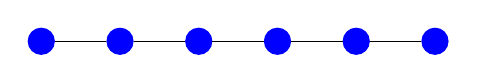
\begin{tikzpicture}
            \foreach \x in {0,...,5} {
                    \node[circle, draw=blue, fill=blue] (\x0) at (\x, 0) {};
                }
            
            \foreach \x [remember=\x as \lastx (initially 0)] in {1,...,5} {
                    \draw (\lastx0) to[] node[left]{}(\x0);
                }
        \end{tikzpicture}
        \\
        Diameter = $N-1$
    \end{center}
\end{defi}

\begin{defi}{Torus oder Ring}
    \begin{center}
        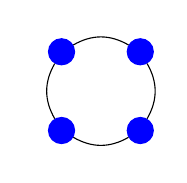
\begin{tikzpicture}
            \node[circle, draw=blue, fill=blue] (d0) at (0, 0) {};
            \node[circle, draw=blue, fill=blue] (d1) at (0, 1) {};
            \node[circle, draw=blue, fill=blue] (d2) at (1, 1) {};
            \node[circle, draw=blue, fill=blue] (d3) at (1, 0) {};
            \draw (d0) to[bend left] node[left]{}(d1);
            \draw (d1) to[bend left] node[left]{}(d2);
            \draw (d2) to[bend left] node[left]{}(d3);
            \draw (d3) to[bend left] node[left]{}(d0);
        \end{tikzpicture}
        \\
        Diameter = $\frac{N}{2}$
    \end{center}
\end{defi}

\begin{defi}{Torus}
    2D-Torus:
    \begin{center}
        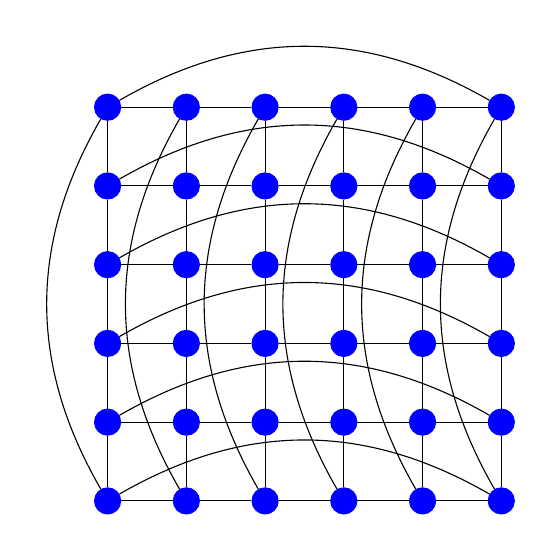
\begin{tikzpicture}[circlestyle/.style={circle, draw=blue, fill=blue}]
            \foreach \x in {0, ..., 5} {
                    \foreach \y in {0, ..., 5} {
                            \node[circlestyle] (\x\y) at (\x, \y) {};
                        }
                }
            
            \foreach \x in {0,...,5}{
                    \foreach \y [count=\yi] in {0,...,4}{
                            \draw (\x\y)--(\x\yi) (\y\x)--(\yi\x); 
                        }
                }
            
            \foreach \x in {0,...,5} {
                    \draw (\x0) to[bend left] node[left]{}(\x5);
                }
            \foreach \y in {0,...,5}{
                    \draw (0\y) to[bend left] node[left]{}(5\y);
                }
        \end{tikzpicture}
        \\
        Diameter = $\sqrt{N}$
    \end{center}
\end{defi}

\begin{defi}{Gitter}
    2D-Gitter:\\
    \begin{center}
        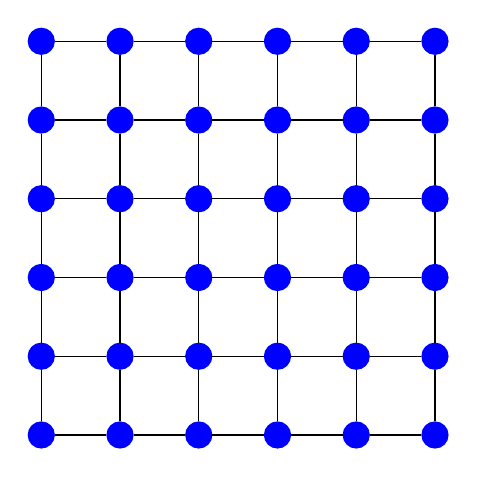
\begin{tikzpicture}[circlestyle/.style={circle, draw=blue, fill=blue}]
            \foreach \x in {0, ..., 5}{
                    \foreach \y in {0, ..., 5}{
                            \node[circlestyle] (\x\y) at (\x, \y) {};
                        }
                }
            
            \foreach \x in {0,...,5}{
                    \foreach \y [count=\yi] in {0,...,4}{
                            \draw (\x\y)--(\x\yi) (\y\x)--(\yi\x); 
                        }
                }
        \end{tikzpicture}
        \\
        Diameter = $2\cdot\left(\sqrt{N} - 1\right)$
    \end{center}
\end{defi}

\begin{defi}{Hypercube}
    \begin{itemize}
        \item Anzahl der Knoten: $N = 2d$
        \item Diameter: $d = \log_2 N$
        \item Greycode Adressierung: Jeder Knoten verbunden mit $d$ anderen Knoten unterscheidet sich durch \emph{ein Bit} in der Adresse
        \item Beispiele: Intel iPSC und NCUBE
        \item Visualisierungen: \\
              \begin{tabular}{|c|c|c|c|}
                  \hline
                  
\begin{tikzpicture}[circlestyle/.style={circle, draw=blue, fill=blue}]
                      \node[circlestyle] (A) at (0,0) {};
                  \end{tikzpicture} & 
                  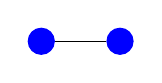
\begin{tikzpicture}[circlestyle/.style={circle, draw=blue, fill=blue}]
                      \node[circlestyle] (A) at (0,0) {};
                      \node[circlestyle] (B) at (1,0) {};
                      \draw (A) -- (B);
                  \end{tikzpicture} & 
                  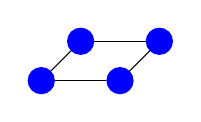
\begin{tikzpicture}[circlestyle/.style={circle, draw=blue, fill=blue}]
                      \node[circlestyle] (A) at (0,0) {};
                      \node[circlestyle] (B) at (1,0) {};
                      \draw (A) -- (B);
                      
                      \node[circlestyle] (C) at (0.5, 0.5) {};
                      \node[circlestyle] (D) at (1.5, 0.5) {};
                      \draw (C) -- (D);
                      
                      \draw (A) -- (C);
                      \draw (B) -- (D);
                  \end{tikzpicture} & 
                  TODO: tikzpicture                         \\
                  \hline
                  0d                         & 1d & 2d & 4d \\
                  \hline
              \end{tabular}
    \end{itemize}
\end{defi}

\begin{defi}{Baum}
    \begin{tabularx}{\textwidth}{|X|X|}
        \toprule
        Planares Layout: & Fetter Baum: (mehr Verbindungen erhöhen das Datenvolumen) \\
        \midrule
        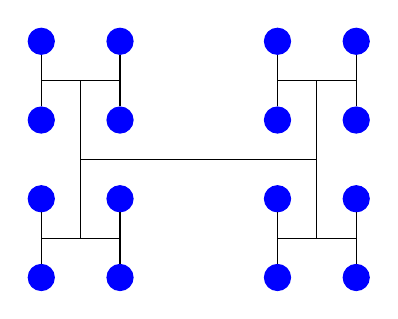
\begin{tikzpicture}[circlestyle/.style={circle, draw=blue, fill=blue}]
            \foreach \y in {0, ..., 3}{
                    \node[circlestyle] (0\y) at (0,\y) {};
                    \node[circlestyle] (1\y) at (1,\y) {};
                    \node[circlestyle] (3\y) at (3,\y) {};
                    \node[circlestyle] (4\y) at (4,\y) {};
                }
            % Connections between nodes
            \draw (00) -- (01);
            \draw (10) -- (11);
            \draw (30) -- (31);
            \draw (40) -- (41);
            
            \draw (02) -- (03);
            \draw (12) -- (13);
            \draw (32) -- (33);
            \draw (42) -- (43);
            %%%
            % Connections between connections
            \draw (0, 0.5) -- (1, 0.5);
            \draw (3, 0.5) -- (4, 0.5);
            
            \draw (0, 2.5) -- (1, 2.5);
            \draw (3, 2.5) -- (4, 2.5);
            
            \draw (0.5, 0.5) -- (0.5, 2.5);
            \draw (3.5, 0.5) -- (3.5, 2.5);
            
            \draw (0.5, 1.5) -- (3.5, 1.5);
            %%%
        \end{tikzpicture}
                         & 
        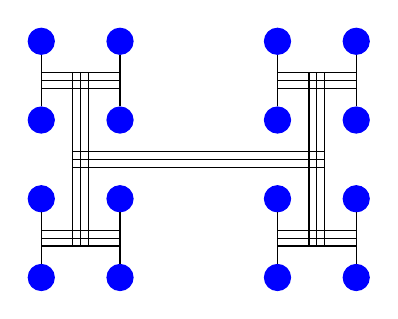
\begin{tikzpicture}[circlestyle/.style={circle, draw=blue, fill=blue}]
            \foreach \y in {0, ..., 3}{
                    \node[circlestyle] (0\y) at (0,\y) {};
                    \node[circlestyle] (1\y) at (1,\y) {};
                    \node[circlestyle] (3\y) at (3,\y) {};
                    \node[circlestyle] (4\y) at (4,\y) {};
                }
            % Connections between nodes
            \draw (00) -- (01);
            \draw (10) -- (11);
            \draw (30) -- (31);
            \draw (40) -- (41);
            
            \draw (02) -- (03);
            \draw (12) -- (13);
            \draw (32) -- (33);
            \draw (42) -- (43);
            %%%
            % Connections between connections
            \draw (0, 0.4) -- (1, 0.4);
            \draw (0, 0.5) -- (1, 0.5);
            \draw (0, 0.6) -- (1, 0.6);
            
            \draw (3, 0.4) -- (4, 0.4);
            \draw (3, 0.5) -- (4, 0.5);
            \draw (3, 0.6) -- (4, 0.6);
            
            \draw (0, 2.4) -- (1, 2.4);
            \draw (0, 2.5) -- (1, 2.5);
            \draw (0, 2.6) -- (1, 2.6);
            
            \draw (3, 2.4) -- (4, 2.4);
            \draw (3, 2.5) -- (4, 2.5);
            \draw (3, 2.6) -- (4, 2.6);
            
            \draw (0.4, 0.4) -- (0.4, 2.6);
            \draw (0.5, 0.4) -- (0.5, 2.6);
            \draw (0.6, 0.4) -- (0.6, 2.6);
            
            \draw (3.4, 0.4) -- (3.4, 2.6);
            \draw (3.5, 0.4) -- (3.5, 2.6);                            
            \draw (3.6, 0.4) -- (3.6, 2.6);
            
            \draw (0.4, 1.4) -- (3.6, 1.4);
            \draw (0.4, 1.5) -- (3.6, 1.5);
            \draw (0.4, 1.6) -- (3.6, 1.6);
            
            %%%
        \end{tikzpicture}
        \\
        \bottomrule
    \end{tabularx}
    \begin{center}
        Diameter = $\log_2 N$
    \end{center}
\end{defi}

\begin{bonus}{Übersicht statischer Verbindungsnetzwerke}
    \begin{tabularx}{\textwidth}{|l|X|X|X|}
        \toprule
        Topologie          & Anzahl der Verbindungskanäle pro Knoten & Maximale Entfernung (Diameter) & Gesamtanzahl der Verbindungskanäle \\
        \midrule
        Ring               & 2                                       & $\frac{N}{2}$                  & $N-1$                              \\
        \midrule
        Baum               & 3                                       & $2\cdot (\log_2 N - 1)$        & $N-1$                              \\
        \midrule
        2D - Gitter        & 4                                       & $2\cdot \sqrt{N}$              & $2\cdot N$                         \\
        \midrule
        3D - Gitter        & 6                                       & $3\cdot \sqrt[3]{N}$           & $3\cdot N$                         \\
        \midrule
        Hexagon. Gitter    & 6                                       & $3\cdot \sqrt[3]{N}$           & $3\cdot N$                         \\ 
        \midrule
        Hypercube          & $\log_2 N$                              & $\log_2 N$                     & $N \log_2 \frac{N}{2}$             \\
        \midrule
        Vollst. Vernetzung & $N - 1$                                 & 1                              & $N \cdot \frac{N-1}{2}$            \\
        \bottomrule
    \end{tabularx}
\end{bonus}

\subsubsection{Dynamische Verbindungsnetzwerke}

\begin{defi}{Bus}
    \begin{itemize}
        \item Durch die wahlweise Zuschaltung einzelner Verarbeitungsknoten zum Datentransfer an einen Bus ist das Bussystem eine typische dynamische Verbindungseinrichtung
        \item Der Bus bildet die Engstelle im busgekoppelten Multiprozessorsystem,
              so dass auch Doppelbusse oder allgemein Mehrfachbusse eingesetzt werden
        \item Bussysteme und auch Mehrbussysteme werden für Systeme mit höchstens 30 Prozessoren eingesetzt,
              um Zugiffskonflikte in Grenzen zu halten
    \end{itemize}
\end{defi}

\begin{defi}{Crossbar}
    \begin{itemize}
        \item $M \times M$ Matrix
        \item einfaches Weiterleiten an mehrere Ausgänge
        \item komplexe Steuerung
        \item Verdrahtungsaufwand
        \item Pufferung bei Blockierungen
        \item Diameter = 1, d. h. beliebige Verbindungen können unter Einsatz jeweils nur einer Schaltzelle realisiert werden
    \end{itemize}
\end{defi}

\begin{defi}{Zellenbasierte Systeme}
    Zellen mit 2 Eingängen und 2 Ausgägen bilden die Basis für solche Systeme.
    \begin{itemize}
        \item 2 Bit $\to$ 4 Schaltzustände
        \item gerade Zellen
        \item kreuzende Zellen
        \item Eingänge mit mehreren Ausgängen verbunden (seltener genutzt)
    \end{itemize}
\end{defi}

\begin{defi}{Einstufige Netzwerke}
    Eine Spalte von Schaltzellen wird durch Rückkopplung der Ausgänge auf die Eingänge Verbunden. 
    Die Zellen werden mehrfach durchlaufen.
\end{defi}

\begin{defi}{Mehrstufige Netzwerke}
    Mehrere Spalten von Schaltzellen, auch mit Rückführungen, 
    sind fest miteinander verbunden.
\end{defi}

\begin{defi}{Omega-Netzwerk}
    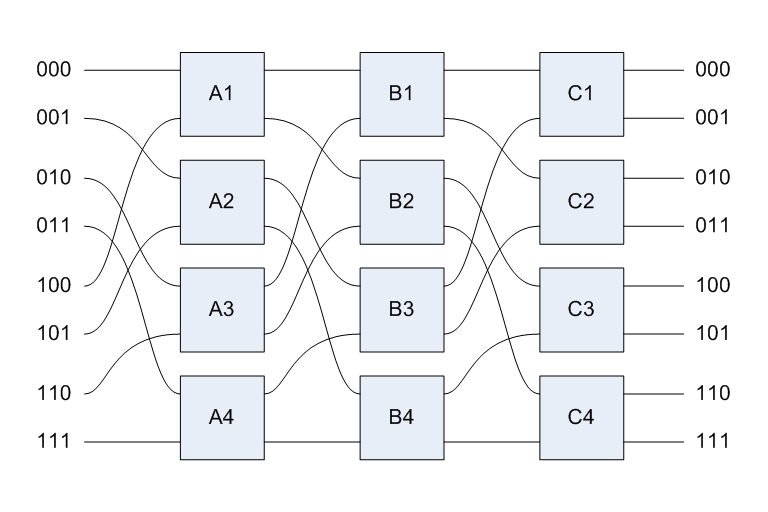
\includegraphics[width=\textwidth]{images/OmegaNetwork.jpg}
    By Bjmyers17, CC BY-SA 3.0, \url{https://commons.wikimedia.org/w/index.php?curid=75639225}
\end{defi}

\begin{defi}{Benes-Netzwerk}
    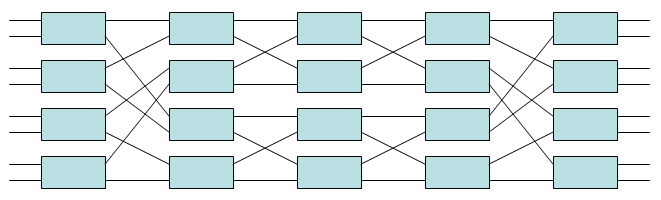
\includegraphics[width=\textwidth]{images/Benesnetwork.png}
    By Piggly - Own work, Public Domain, \url{https://commons.wikimedia.org/w/index.php?curid=2988080}
\end{defi}

\begin{defi}[Cluster-Interconnect]{Infiniband}
    Infiniband \ldots
    \begin{itemize}[\ldots]
        \item ist eine Architektur für Hochgeschwindigkeitsverbindungen zwischen Rechnern und externen Speicherservern.
        \item wurde unter Führung von Intel entwickelt, später Mellanox, jetzt Nvidia.
        \item eignet sich auch als Verbindungsnetzwerk von Rechen-Clustern.
    \end{itemize}
    aktuell: Infiniband EDR / HDR mit bis zu 200 Gbit/s
\end{defi}

\begin{defi}[Cluster-Interconnect]{Gigabit Ethernet}
    Gigabit Ethernet \ldots
    \begin{itemize}[\ldots]
        \item wird vorwiegend in lokalen Netzwerken genutzt,
              auch für Heimanwender mit RJ45 Stecker für Kupferkabel (z.B. Lan-Buchsen am Router)
        \item ist für Glasfaser und (twisted-pair) Kupferkabel spezifiziert,
              höhrere Bandbreiten aber nur über Glasfaser umsetzbar: bis zu 100 Gb/s
        \item ist Switch-basiert und abwärtskompatibel
        \item nutzt spezielle Kollisionserkennung / -vermeidung,
              wie CSMA / CD (Carrier Sense Multiple Access with Collision Detection)
    \end{itemize}
\end{defi}

\begin{defi}[Verbindungsnetzwerk]{Klassifikation}
    \begin{center}
        \begin{forest}for tree={inner sep=2pt,outer sep=0pt,align=center,font=\sffamily\footnotesize,draw}
            [Verbindungsnetzwerk
                [statisch
                        [ein-\\dimensional]
                        [zwei-\\dimensional]
                        [mehr-\\dimensional]
                ]
                [dynamisch
                        [Bussysteme]
                        [Zellenbasierte \\ Netze
                                [einstufig]
                                [mehrstufig
                                        [blockierend]
                                        [nicht-blockierend]
                                ]
                        ]
                        [Kreuzschienenverteiler \\ (Crossbars)]
                ]
            ]
        \end{forest}
    \end{center}
\end{defi}

\subsection{Cache-Kohärenz}

\begin{defi}{Cache-Kohärenz}
    \begin{itemize}
        \item wichtig bei Mehrprozessorsystemen mit Shared-Memory oder Shared Virtual Memory $\to$ SMP
        \item Maßnahmen zur Verhinderung von unterschiedlichen Versionen der gleichen Cache-Zeile in 2 oder mehreren Caches
        \item Technische Lösungen:
              \begin{itemize}
                  \item \emph{Snooping Caches} (auf den Leitungen den Datenverkehr ausschnüffeln == to snoop) $\to$ Bus-basierte Systeme
                  \item \emph{Directory-basierte Caches} $\to$ komplexere Verbindungsnetze
              \end{itemize}
    \end{itemize}
\end{defi}

\begin{defi}[Cache-Kohärenz]{Snooping Cache Protocols}
    Es gibt mehrere Snoopy-Protokolle (z.B. MESI). 
    Sie basieren auf der \enquote{Invalidate}-Strategie:
    \begin{itemize}
        \item beim Schreiben von \enquote{shared data} wird ein \enquote{invalidate}-Signal an alle anderen Caches gesendet,
              die eine Kopie dieses Datums als ungültig kennzeichnen
        \item beim Lesen kann jeder Prozessor seine gültige Version der Cache-Zeile verwenden
        \item findet ein Prozessor beim Lesen kein gültiges Datum: Read-Miss
              \begin{itemize}
                  \item bei \enquote{write-through}-Caches befindet sich das Memory immer im aktuellen Zustand:
                        Datum wird in den anfordernden Cache gelesen
                  \item bei \enquote{write-back}-Caches:
                        suche (snoop) in den anderen Caches nach einer gültigen Version
              \end{itemize}
    \end{itemize}
\end{defi}

\begin{defi}[Cache-Kohärenz]{Directory-basierte Caches}
    Bus-basierte Snooping-Protokolle skalieren nicht bei großen Netzwerken mit NUMA-Architektur 
    $\to$ Directory-Protokolle $\to$ ccNUMA \\
    Directory-basierte Protokolle sind ähnlich zu Snoopy-Protokoll.
    Das Directory hat ein Zustandsfeld mit 3 möglichen Zuständen:
    \begin{itemize}
        \item \emph{Shared:}     $\geq$ 1 Prozessor besitzen Daten, Memory aktuell
        \item \emph{Uncached:}   Kein Prozessor (kein Cache) besitzt gültige Daten
        \item \emph{Exclusive:}  1 Prozessor (owner) besitzt die Daten, Memory nicht aktuell
    \end{itemize}
\end{defi}

\subsection{Aufgaben}

\begin{aufgabe}{Multiprozessoren}
    Nennen Sie zwei verschiedene Arten von nachrichtengekoppelten Multiprozessoren.
    \tcblower
    \begin{itemize}
        \item Massively Parallel Processor (MPP)
        \item Cluster Of Workstation (COW)
    \end{itemize}
\end{aufgabe}

\begin{aufgabe}{Multiprozessoren}
    Welche beiden Arten von speichergekoppelten Multiprozessor-Systemen wurden in der Vorlesung unterschieden?
    \tcblower
    \begin{itemize}
        \item Uniform Memory Access (UMA)
        \item Non Uniform Memory Access (NUMA)
    \end{itemize}
\end{aufgabe}

\begin{aufgabe}{Multiprozessoren}
    Zwischen welchen speichergekoppelten Multiprozessoren unterscheidet man je nach physikalischer Speicherorganisation?
    \tcblower
    \begin{itemize}
        \item Symmetric multiprocessor (SMP)
        \item Distributed shared memory Systeme
    \end{itemize}
\end{aufgabe}

\begin{aufgabe}{Distributed Memory Machines}
    Auf welche beiden Arten kann eine Distributed Memory Machine realisiert werden?
    \tcblower
    \begin{itemize}
        \item speichergekoppelt als shared virtual memory (SVM) $\to$ NUMA
        \item nachrichtengekoppelt (z.B. Cray T3E)
    \end{itemize}
\end{aufgabe}

\begin{aufgabe}{Verbindungsnetzwerk}
    Nennen und erklären Sie kurz die fünf grundlegenden Eigenschaften eines Verbindungsnetzwerkes.
    \tcblower
    \begin{tabularx}{\textwidth}{|X|X|}
        \toprule
        Eigenschaft            & Erklärung                                                                                                                                                    \\
        \midrule
        Latenz (latency)       & Zeit für den Transfer zwischen den Knoten                                                                                                                    \\
        \midrule
        Bandbreite (bandwidth) & $\frac{\text{transferierte Daten}}{Zeit}$, \newline Bandbreite eines Link: $\text{bw} = \omega \cdot \frac{1}{t} \left(\frac{\text{bit}}{\text{sec}}\right)$ \\
        \midrule
        Diameter               & maximale Distanz zwischen zwei beliebigen Prozessoren                                                                                                        \\
        \midrule
        Topologie              & wie sind die Nachbarknoten angeordnet und erreichbar                                                                                                         \\
        \midrule
        Statische oder \newline dynamische Leitungswege                                                                                                                                       \\
        \bottomrule
    \end{tabularx}
\end{aufgabe}

\begin{aufgabe}{Verbindungsnetzwerk}
    Nennen Sie drei unterschiedliche Verbindungsnetzwerk-Topologien.
    \tcblower
    \begin{itemize}
        \item Torus
        \item (Hyper)cube / Mesh
        \item Tree / Fat Tree
    \end{itemize}
\end{aufgabe}

\begin{aufgabe}{Verbindungsnetzwerk}
    Durch welche physikalische Maßnahme kann bei einem Tree-Netzwerk der Durchsatz erhöht werden?
    \tcblower
    Man erstellt eine zunehmende Anzahl an Leitungen zur Wurzel hin ($\to$ Fat Tree).
\end{aufgabe}

\begin{aufgabe}{Verbindungsnetzwerk}
    Wie groß ist der Durchmesser eines 2D Torus mit N Gitterpunkten?
    \tcblower
    $$\sqrt{N}$$
\end{aufgabe}

\begin{aufgabe}{Verbindungsnetzwerk}
    Was sind die zwei gebräuchlichsten Netzwerktypen im HPC-Bereich?
    \tcblower
    \begin{itemize}
        \item Gbit Ethernet
        \item Infiniband
    \end{itemize}
\end{aufgabe}

\begin{aufgabe}{Cache-Kohärenz}
    Bei Mehrprozessorsystemen mit welchem Speicher ist Cache-Kohärenz wichtig?
    \tcblower
    \begin{itemize}
        \item Shared Memory
        \item Shared Virtual Memory
    \end{itemize}
\end{aufgabe}

\begin{aufgabe}{Cache-Kohärenz}
    Geben Sie zwei technische Lösungen an, um Cache-Kohärenz herzustellen.
    \tcblower
    \begin{itemize}
        \item Snooping Caches
        \item Directory-basierte Systeme
    \end{itemize}
\end{aufgabe}

\begin{aufgabe}{Cache-Kohärenz}
    Durch welches Hilfsmittel kann in Bus-basierten Systemen mit \enquote{write-back}-Caches Cache-Kohärenz realisiert werden?
    \tcblower
    Snoopy-Protokolle
\end{aufgabe}

\begin{aufgabe}{Cache-Kohärenz}
    Auf welcher Strategie basieren Snoopy-Protokolle?
    \tcblower
    Invalidate Strategie
\end{aufgabe}

\begin{aufgabe}{Cache-Kohärenz}
    Womit lässt sich Cache-Kohärenz bei Distributed Memory Systemen realisieren?
    \tcblower
    Directory basierte Protokolle
\end{aufgabe}

\begin{aufgabe}{Cache-Kohärenz}
    Wie lauten die drei möglichen Zustände des Zustandsfeldes der Directory bei einem Directory-basierten Protokoll?
    \tcblower
    \begin{itemize}
        \item Shared: $\geq$ 1 Prozessor besitzen Daten, Memory aktuell
        \item Uncached: Kein Prozessor (kein Cache) besitzt gültige Daten
        \item Exclusive: 1 Prozessor (owner) besitzt die Daten, Memory nicht aktuell
    \end{itemize}
\end{aufgabe}